% Chapter 2: Methods
\chapter{Methods}
\section{Data Collection}
\begin{figure}[h!]
    \centering
    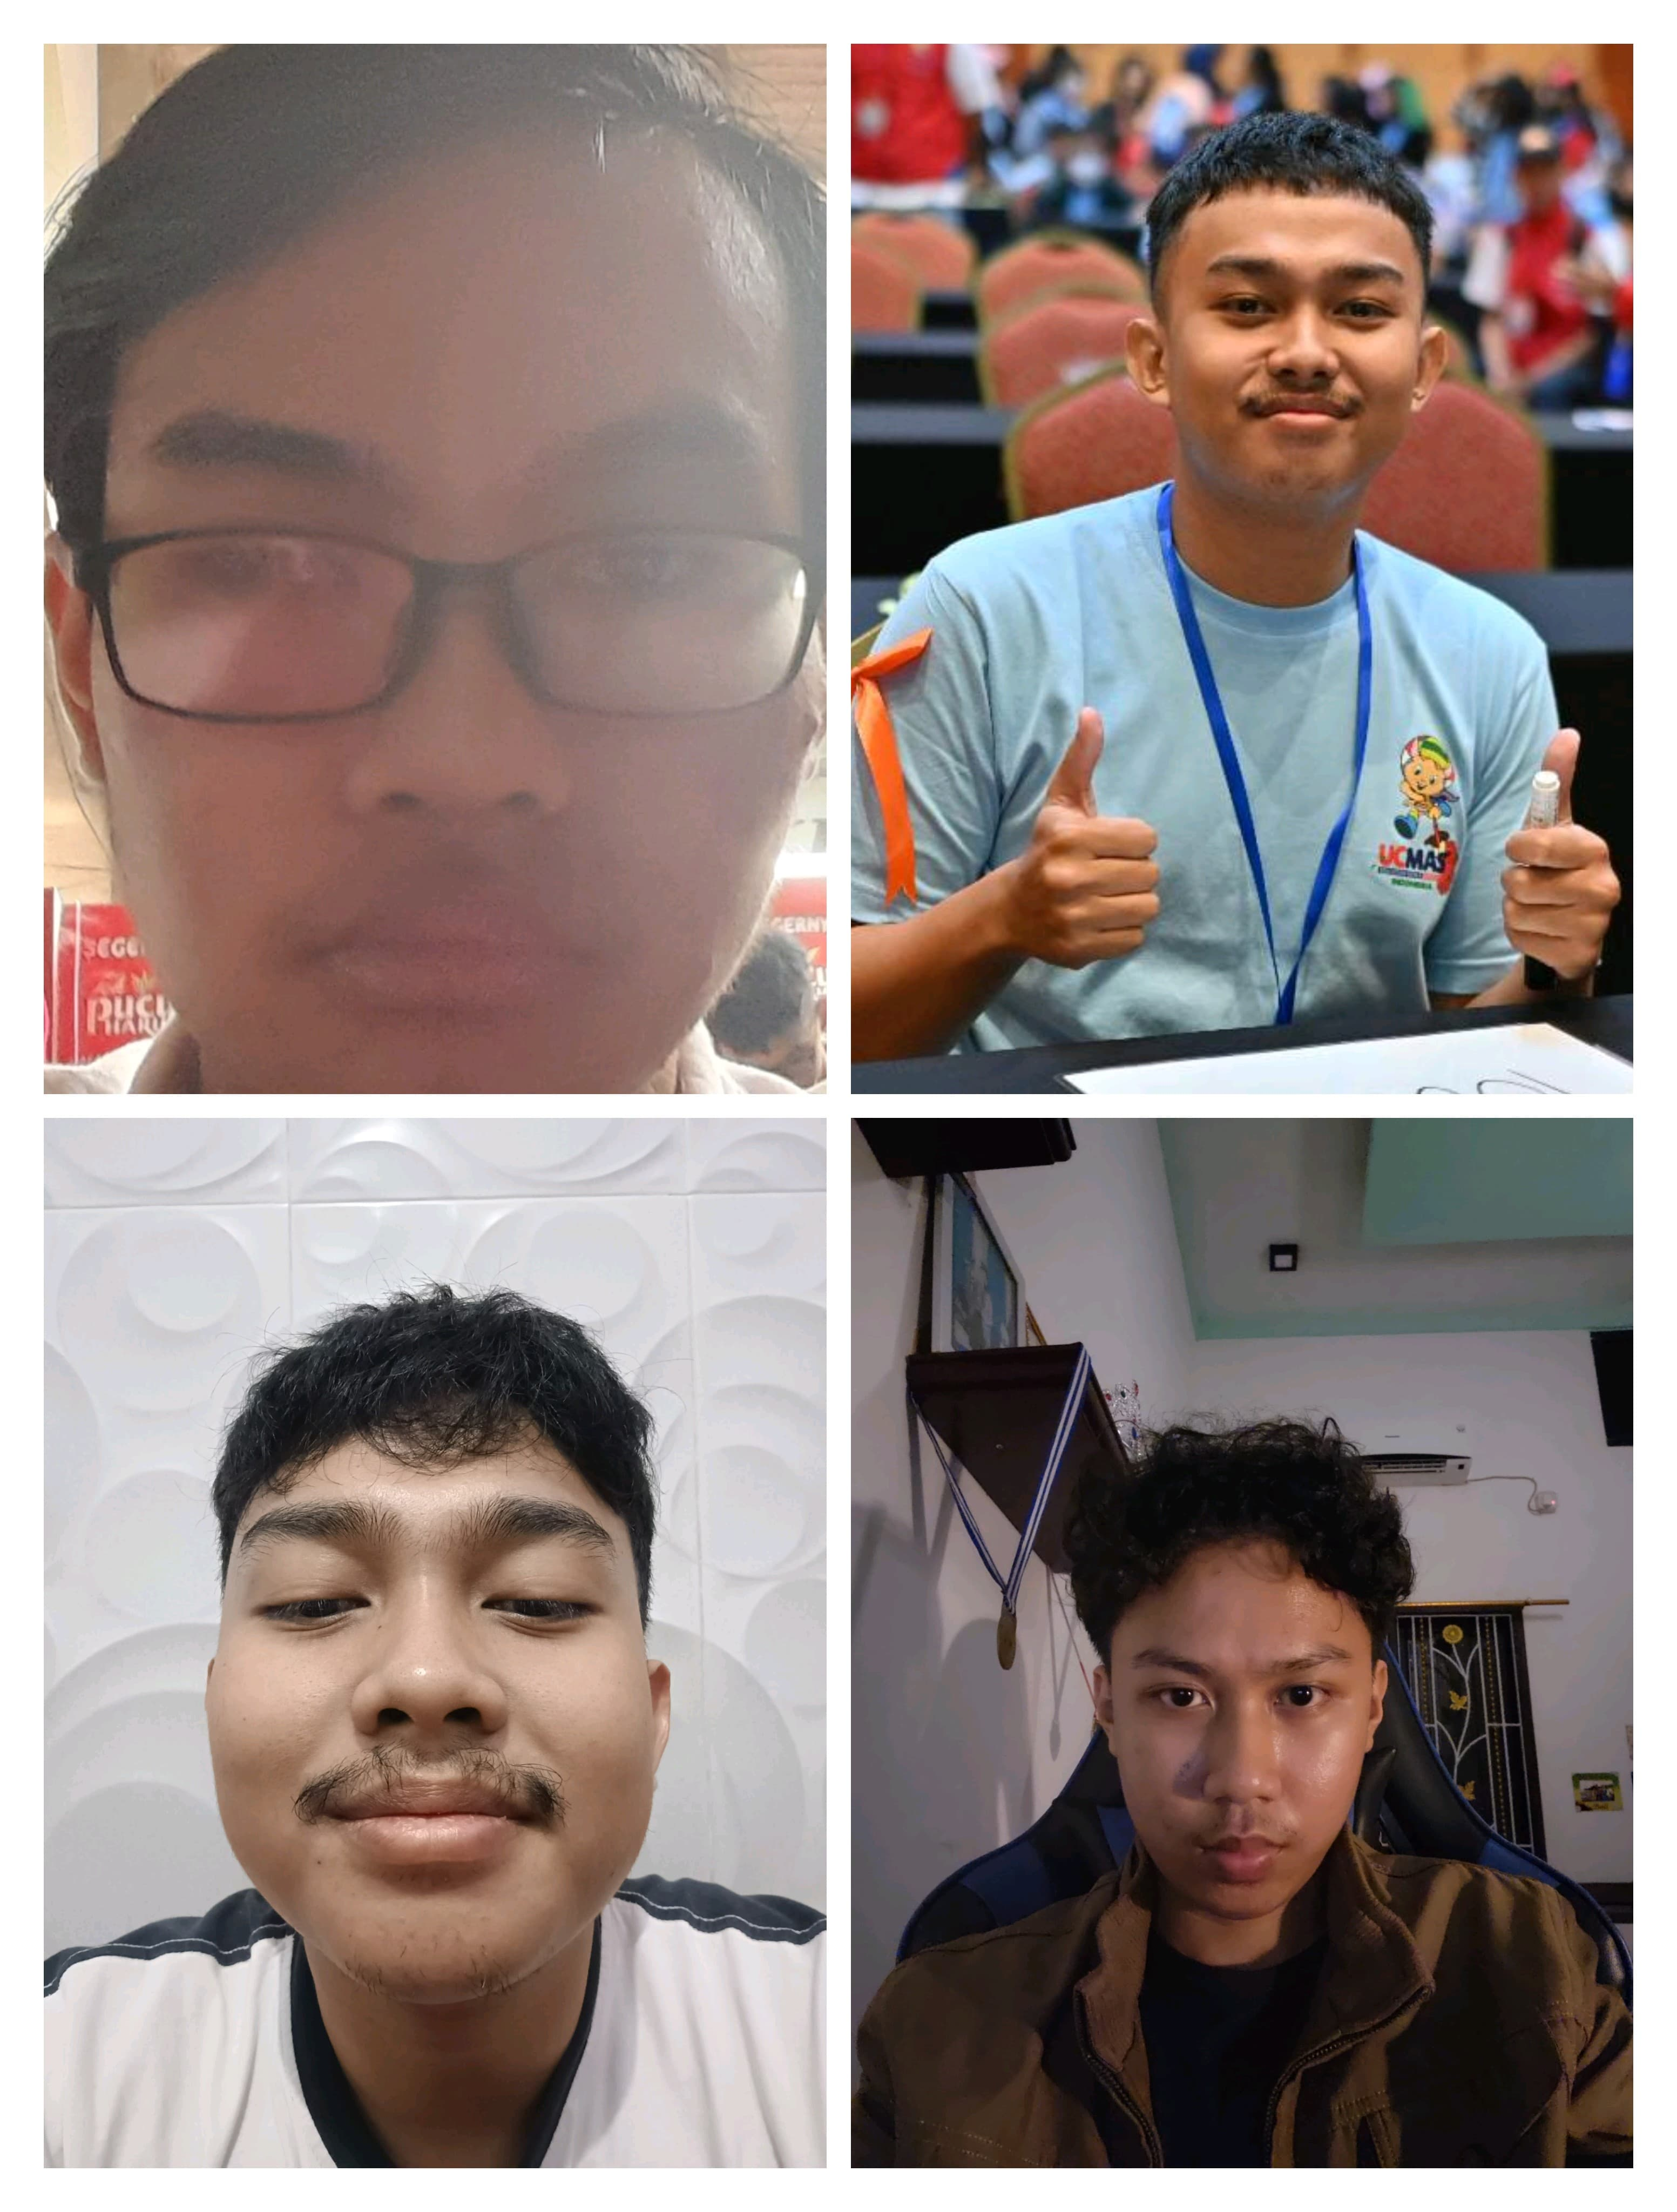
\includegraphics[width=0.5\textwidth]{images/img_source_example.jpeg}
    \caption{Image captured example}
    \label{fig:ex_photo}
\end{figure}

The data for the face recognition-based attendance application was collected from multiple sources to ensure the model's ability to recognize student faces in real-world classroom conditions. We used two primary methods for data collection:
\subsection{Manual Image Capture}
Several images of our team member faces were manually captured using a camera in various lighting conditions and backgrounds. These images were collected to ensure the dataset includes faces in both ideal and suboptimal conditions(see Figure \ref{fig:ex_photo}).
\subsection{Video Frame Extraction}
In addition to manually captured images, we also utilized a video frame extraction technique. Videos were recorded in classroom environments, and frames were extracted from the videos to increase the dataset's size. This method also allows for the inclusion of multiple facial images from different angles, poses, and expressions.
\subsection{Image Labeling with Roboflow}
After gathering the images, we used Roboflow, a popular image annotation tool, to label the dataset. Roboflow enabled us to efficiently label each image with the corresponding student’s identity, creating a structured dataset for training the face recognition model. With Roboflow, we were able to organize the images into different classes, each representing our team member (see Figure \ref{fig:roboflow_combined}).

\begin{figure}[h!]
    \centering
    \begin{subfigure}[b]{0.55\textwidth}
        \centering
        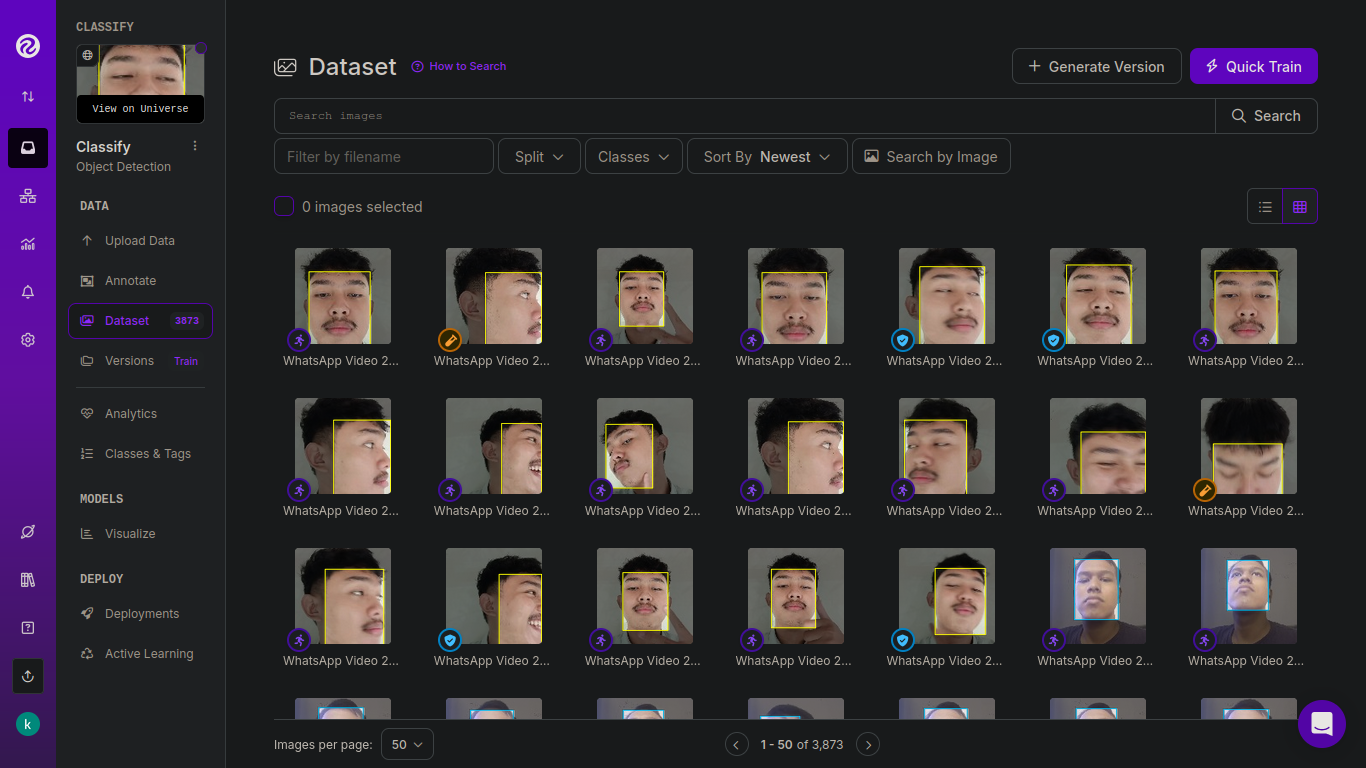
\includegraphics[width=\textwidth]{images/roboflow_ss.png}
        \caption{Roboflow interface for list of annotated and unannotated images}
        \label{fig:ex_roboflow}
    \end{subfigure}
    \hfill
    \begin{subfigure}[b]{0.35\textwidth}
        \centering
        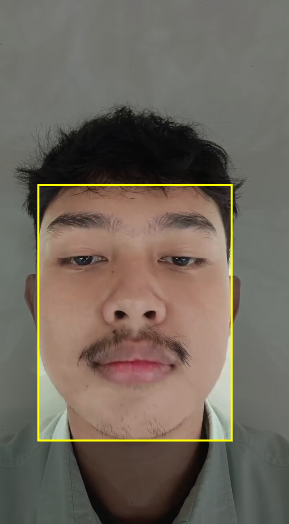
\includegraphics[width=\textwidth]{images/labeling process.png}
        \caption{Roboflow interface for image labeling process}
        \label{fig:roboflow_process}
    \end{subfigure}
    \caption{Roboflow interface: (a) Annotation list view, (b) Labeling process view}
    \label{fig:roboflow_combined}
\end{figure}

\section{Data Explanation}
The dataset used for the attendance system consists of facial images of students, each assigned a label corresponding to a unique student identity. The key features of the dataset are outlined as follows:
\subsection{Images}
Each image is stored in a common format such as JPEG or PNG, with varying resolutions ranging from 640x640 pixels to 720x1920 pixels. The images were captured to ensure the facial features are clear and can be accurately recognized by the model.
\subsection{Classes and Labels}
Each student in the dataset is represented as a separate class, with each image assigned to a corresponding label. There are between 638 and 661 labeled images for each team member, based on the number of images available. The labels, which were generated using Roboflow, allow the model to learn to distinguish between different team member by identifying their unique facial features.
\subsection{Conditions of Image Capture}
The images in the dataset were taken under a variety of conditions to simulate real-world classroom environments. These include low-light conditions, outdoor environments, and images taken at low resolutions. These diverse conditions ensure that the model can recognize faces in less-than-ideal situations, such as varying lighting or poor image quality.
\subsection{Preprocessing}
Once labeled, the images underwent preprocessing before being used for model training. This included resizing the images to a standard resolution and normalizing pixel values to maintain consistency. Additionally, data augmentation techniques such as random rotations and zooms were applied to enhance the dataset and make the model more robust to different face angles and expressions

\section{Algorithm or Model}
For this project, we utilized the YOLOv8 model for face recognition and detection. YOLO (You Only Look Once) is a convolutional neural network known for its accuracy and speed in object detection tasks, making it suitable for real-time applications such as face recognition. The model was trained using a dataset of labeled faces to allow it to distinguish individual team members. We used the medium variant of YOLOv8, which balances accuracy and computational efficiency, making it a good choice for our dataset size and target application.

\begin{verbatim}
    import os
    from ultralytics import YOLO

    model = YOLO("yolov8m.pt")
    
    train_results = model.train(data="data.yaml", epochs=100, imgsz=640)
\end{verbatim}

\section{Testing}
\subsection{Testing Procedures}
The testing process for the Classify App focuses on validating the model’s accuracy, functionality, and security compliance. Specific scenarios, such as low-light conditions, angled views, and multiple faces in a frame, are incorporated to assess the system’s performance. Procedures include functional verification of features like registration, login, and attendance recognition, ensuring each works as expected across different device and environmental conditions.

\subsection{Testing Metrics}
Key testing metrics, including accuracy, precision, and compliance with security standards, are measured to assess the model's performance. Accuracy metrics gauge the model’s reliability across diverse lighting and angle variations, while security tests validate data encryption during capture and storage. These metrics provide insight into both functional performance and data safety.

\section{Evaluation Metrics}
Evaluation metrics encompass recognition accuracy, processing speed, and resilience under varied conditions. Accuracy is measured to ensure an 85% threshold in recognition even in challenging conditions like low light. Speed metrics are evaluated to confirm real-time usability, and reliability is assessed by verifying the system’s consistency in handling multiple faces or varied conditions. Together, these metrics ensure the Classify App meets its intended performance and security standards in practical, real-world scenarios.


